\documentclass[11pt]{article}
\usepackage{amsmath,amsbsy,amssymb,verbatim,fullpage,ifthen,graphicx,bm,amsfonts,amsthm}
\usepackage{graphicx}
\usepackage{xcolor}
\usepackage{hyperref}
\usepackage{booktabs}
\usepackage{multicol}
\usepackage{algorithm}
\usepackage{algorithmic}
\usepackage{algpseudocode}
\newcommand{\mfile}[1]  {{\small \verbatiminput{./#1}}} % Jeff Fessler, input matlab file
\newcommand{\tmop}[1]{\ensuremath{\operatorname{#1}}}

\newcommand{\R}{\mathbb{R}}
\newcommand{\C}{\mathbb{C}}
\newcommand{\Z}{\mathbb{Z}}
\newcommand{\A}{\mathcal{A}}
\newcommand{\minimize}{\operatorname*{minimize\ }}
\newcommand{\maximize}{\operatorname*{maximize}}

%\newcommand{\mfile}[1]  {{\small \verbatiminput{./#1}}} 
\newcommand{\mtx}[1]{\mathbf{#1}}
\newcommand{\vct}[1]{\mathbf{#1}}
\def \lg       {\langle}
\def \rg       {\rangle}
\def \mA {\mtx{A}}
\def \mC {\mtx{C}}
\def \mI {\mtx{I}}
\def \mU {\mtx{U}}
\def \mS {\mtx{S}}
\def \mV {\mtx{V}}
\def \mW {\mtx{W}}
\def \mLambda {\mtx{\Lambda}}
\def \mX {\mtx{X}}
\def \mY {\mtx{Y}}
\def \mZ {\mtx{Z}}
\def \zero     {\mathbf{0}}
\def \vzero    {\vct{0}}
\def \vone    {\vct{1}}
\def \vu {\vct{u}}
\def \vv {\vct{v}}
\def \vx {\vct{x}}
\def \vy {\vct{y}}
\def \vz {\vct{z}}
\def \vphi {\vct{\phi}}
\def \vmu {\vct{\mu}}
\def \R {\mathbb{R}}

\usepackage{listings}

\lstset{
  language=Python,
  basicstyle=\ttfamily\small,
  keywordstyle=\color{blue},
  commentstyle=\color{gray},
  stringstyle=\color{red},
  frame=single,
  breaklines=true,
  showstringspaces=false
}

\usepackage{xspace}

\makeatletter
\DeclareRobustCommand\onedot{\futurelet\@let@token\@onedot}
\def\@onedot{\ifx\@let@token.\else.\null\fi\xspace}

\def\eg{\emph{e.g}\onedot} \def\Eg{\emph{E.g}\onedot}
\def\ie{\emph{i.e}\onedot} \def\Ie{\emph{I.e}\onedot}
\def\cf{\emph{c.f}\onedot} \def\Cf{\emph{C.f}\onedot}
\def\etc{\emph{etc}\onedot} \def\vs{\emph{vs}\onedot}
\def\wrt{w.r.t\onedot} \def\dof{d.o.f\onedot}
\def\etal{\emph{et al}\onedot} \def\st{\emph{s.t}\onedot}
\pagestyle{plain}

\title{{\bf Homework Set 2, CPSC 6430/4430}}
\author{\Large\underline{Ellis, Michael}}
\date{\textbf{\Large\textcolor{red}{Due 03/13/2026, 11:59PM EST}}}

\begin{document}
\maketitle

\section*{GD for Ridge Regression}

For Ridge Regression: \\

$$
\min _{\mathbf{x}}\|\mathbf{A x}-\mathbf{y}\|_2^2+\gamma\|\mathbf{x}\|_2^2,
$$

\noindent 1. What is the derivative with respect to $\mathbf{x}$? \\\\
2. What is the closed solution of ridge regression? \\\\
3. Assume $\mathbf{A} \in \mathbb{R}^{100 \times 50}$, and stepsize $\lambda=0.5 /\left(\gamma+\sigma_1\left(\mathbf{A A}^T\right)\right)$, where $\sigma_1(\mathbf{Z})$ denotes the largest singular value of $\mathbf{Z}$. Please change $\lambda$ from $\{0.01,0.1,1,10,100\}$ and plot the objective changes with update via gradient descent method (100 iterations), what do you find?


\subsection*{1. Derivative with respect to $\mathbf{x}$}

The ridge regression objective is

\[
f(\mathbf{x}) = \|\mathbf{A}\mathbf{x}-\mathbf{y}\|_2^2 + \gamma \|\mathbf{x}\|_2^2 .
\]

Expanding the terms,

\[
f(\mathbf{x}) =
(\mathbf{A}\mathbf{x}-\mathbf{y})^\top(\mathbf{A}\mathbf{x}-\mathbf{y})
+ \gamma \mathbf{x}^\top \mathbf{x}.
\]

Taking the derivative with respect to $\mathbf{x}$,

\[
\nabla_{\mathbf{x}} f(\mathbf{x})
=
2\mathbf{A}^\top(\mathbf{A}\mathbf{x}-\mathbf{y})
+
2\gamma \mathbf{x}.
\]

\[
\boxed{
\nabla_{\mathbf{x}} f(\mathbf{x})
=
2\mathbf{A}^\top(\mathbf{A}\mathbf{x}-\mathbf{y})
+
2\gamma \mathbf{x}
}
\]

\subsection*{2. Closed-form solution of Ridge Regression}

Setting the gradient to zero,

\[
2\mathbf{A}^\top(\mathbf{A}\mathbf{x}-\mathbf{y}) + 2\gamma \mathbf{x} = 0.
\]

Rearranging,

\[
\mathbf{A}^\top \mathbf{A}\mathbf{x} - \mathbf{A}^\top \mathbf{y} + \gamma \mathbf{x} = 0.
\]

\[
(\mathbf{A}^\top \mathbf{A} + \gamma \mathbf{I})\mathbf{x} = \mathbf{A}^\top \mathbf{y}.
\]

Thus the ridge regression solution is

\[
\boxed{
\mathbf{x}^* =
(\mathbf{A}^\top \mathbf{A} + \gamma \mathbf{I})^{-1}
\mathbf{A}^\top \mathbf{y}
}
\]

\subsection*{3. Gradient Descent Experiment}

Gradient descent updates $\mathbf{x}$ using

\[
\mathbf{x}_{k+1}
=
\mathbf{x}_k
-
\lambda
\left(
2\mathbf{A}^\top(\mathbf{A}\mathbf{x}_k-\mathbf{y})
+
2\gamma \mathbf{x}_k
\right).
\]

The suggested stepsize is

\[
\lambda =
\frac{0.5}{\gamma + \sigma_1(\mathbf{A}\mathbf{A}^\top)}
\]

where $\sigma_1(\mathbf{Z})$ denotes the largest singular value of $\mathbf{Z}$.


after running gradient descent for 100 iterations with different step sizes relative to the recommended safe step size:

\[
\lambda_{\text{safe}} = \frac{1}{2(\sigma_{\max}(A)^2 + \gamma)}.
\]

From the plot we observe the following:

\begin{itemize}

\item All step sizes eventually approach the same objective value, which matches the closed-form ridge regression solution.

\item Smaller step sizes converge more slowly because the updates are small.

\item Step sizes near the safe bound converge significantly faster.

\item If the step size becomes too large, gradient descent becomes unstable and the objective value diverges.

\end{itemize}

This experiment demonstrates the importance of choosing an appropriate step size for gradient descent.

\subsubsection*{Python Code for Gradient Descent Experiment}

\begin{verbatim}
import numpy as np
import matplotlib.pyplot as plt

np.random.seed(0)
m, n = 100, 50
A = np.random.randn(m, n)
y = np.random.randn(m)
gamma = 1.0
iterations = 100

def objective(x):
    r = A @ x - y
    return np.linalg.norm(r)**2 + gamma * np.linalg.norm(x)**2

def gradient(x):
    return 2 * A.T @ (A @ x - y) + 2 * gamma * x

# compute sigma_max(A)
s = np.linalg.svd(A, compute_uv=False)
sigma_max = s[0]
lambda_safe = 1.0 / (2.0 * (sigma_max**2 + gamma))  # stable upper bound

# choose step sizes around the safe value
lambdas = [lambda_safe * f for f in [0.1, 0.5, 1.0, 2.0]]
labels = [f"{f:.1g} * lambda_safe" for f in [0.1, 0.5, 1.0, 2.0]]

results = {}
for lam, lab in zip(lambdas, labels):
    x = np.zeros(n)
    objs = []
    diverged = False
    for it in range(iterations):
        val = objective(x)
        if not np.isfinite(val) or val > 1e100:
            # stop on divergence
            objs.append(np.nan)
            diverged = True
            break
        objs.append(val)
        x = x - lam * gradient(x)
    # pad to uniform length for plotting
    if len(objs) < iterations:
        objs += [np.nan] * (iterations - len(objs))
    results[lab] = np.array(objs)

# closed-form solution objective for reference
x_star = np.linalg.solve(A.T @ A + gamma * np.eye(n), A.T @ y)
f_star = objective(x_star)

plt.figure(figsize=(8,5))
for lab, vals in results.items():
    mask = np.isfinite(vals)
    if mask.any():
        plt.plot(np.arange(len(vals))[mask], vals[mask], label=lab)
# horizontal line for optimal objective
plt.axhline(f_star, linestyle='--', label='closed-form optimum')
plt.yscale('log')
plt.xlabel('Iteration')
plt.ylabel('Objective value (log scale)')
plt.title('GD on Ridge regression (safe step sizes tested)')
plt.legend()
plt.grid(True)
plt.tight_layout()
plt.savefig('ridge_gd_safe.png', dpi=150)
plt.show()
\end{verbatim}

\begin{figure}[h]
\centering
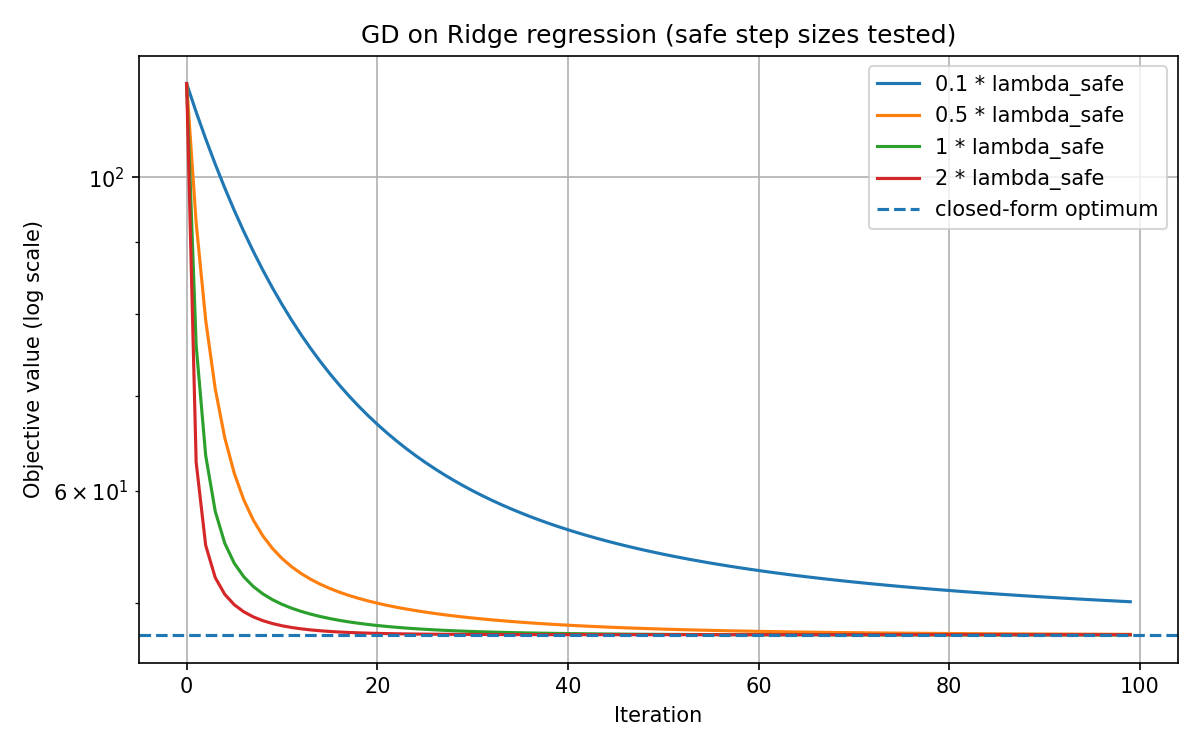
\includegraphics[width=0.7\textwidth]{ridge_gd_safe.png}
\caption{Objective value vs iteration for gradient descent on ridge regression using different step sizes relative to the recommended stepsize $\lambda = \frac{0.5}{\gamma + \sigma_1(AA^T)}$. Smaller step sizes converge more slowly, while step sizes near the recommended value converge faster toward the closed-form optimum.}
\end{figure}

\newpage 

\section*{Optimization for Lasso}

We now turn to discuss Lasso model which is not mentioned in class:

$$
\min _{\mathbf{x}} \frac{1}{2}\|\mathbf{A} \mathbf{x}-\mathbf{y}\|_2^2+\lambda\|\mathbf{x}\|_1,
$$

\noindent where we define $\|\mathbf{z}\|_2^2=\sum\limits_i \mathbf{z}_i^2,\|\mathbf{x}\|_1=\sum\limits_i\left|\mathbf{x}_i\right|$. Different from linear regression or ridge regression, where we can obtain the optimal solution by taking the derivative with respect to $\mathbf{x}$ and set to 0 , the main drawback of Lasso model is $\|\cdot\|_1$ is not differentiable. To address the issue, we turn to a different optimization framework which is summarized as below:

\begin{algorithm}
    \caption{An algorithm to solve Eq. (2)}
    \label{alg:equation2}
    
    \begin{algorithmic}[]
        \STATE $\mathrm{x} \leftarrow 0$ 
        \STATE $t \leftarrow 1 / \sigma_1\left(\mathbf{A A}^T\right)$
        \STATE $k \leftarrow 1$
        \STATE $K \leftarrow 100$ 
        \WHILE $k \leq K$ \DO
            \STATE $\mathbf{z}=\mathbf{x}-t \mathbf{A}^T(\mathbf{A} \mathbf{x}-\mathbf{y})$ \\
            \textit{$* * *$ for each element in $\mathbf{z}$ and $\mathbf{x} * * *$} \\
            \textit{$\mathbf{x}_i=\operatorname{sign}\left(\mathbf{z}_i\right) * \max \left\{\left|\mathbf{z}_i\right|-t \lambda, 0\right\}$}
        \STATE \textbf{end while}
    \end{algorithmic}
\end{algorithm}

\noindent 1. Please implement the algorithm and plot the objective changes with update (for $\lambda=1$ and $\lambda=2$, respectively) where x -axis is the iteration and y -axis is the objective in Eq. (2)). \\\\
2. Please compare the output from Algorithm 1 with Lasso in sklearn and check whether they are close. You can randomly generate $\mathbf{A} \in \mathbb{R}^{100 \times 50}, \mathbf{y} \in \mathbb{R}^{100}$.

\subsection*{Part 1: Implement Algorithm 1}

We implement Algorithm 1 using the ISTA (Iterative Soft Thresholding Algorithm).
At each iteration we perform a gradient step followed by a soft-thresholding
operation to handle the $\ell_1$ regularization.

\begin{verbatim}
# Python implementation of Algorithm 1
# ISTA (Algorithm 1) for Lasso + comparison with sklearn
import numpy as np
import matplotlib.pyplot as plt
from sklearn.linear_model import Lasso

np.random.seed(0)

# Problem size
m, n = 100, 50

# Data (random example)
A = np.random.randn(m, n)
y = np.random.randn(m)

# Parameters
lambdas = [1.0, 2.0]      # lambda values to test
K = 200                   # iterations for ISTA

def objective(A, y, x, lam):
    r = A @ x - y
    return 0.5 * np.linalg.norm(r)**2 + lam * np.linalg.norm(x, 1)

def ista(A, y, lam, K, x0=None):
    m, n = A.shape
    if x0 is None:
        x = np.zeros(n)
    else:
        x = x0.copy()
    # compute sigma1(AA^T) (largest singular value of AA^T)
    sigma1 = np.linalg.svd(A @ A.T, compute_uv=False)[0]
    t = 1.0 / sigma1   # step size as in the algorithm
    objs = []
    for k in range(K):
        # gradient step on smooth part
        grad = A.T @ (A @ x - y)   # gradient of 0.5||Ax-y||^2 is A^T(Ax-y)
        z = x - t * grad
        # soft-thresholding (proximal operator)
        x = np.sign(z) * np.maximum(np.abs(z) - t * lam, 0.0)
        objs.append(objective(A, y, x, lam))
    return x, np.array(objs), t

# Run ISTA and compare with sklearn Lasso
results = {}
for lam in lambdas:
    x_ista, objs, t_used = ista(A, y, lam, K)
    results[lam] = {'x_ista': x_ista, 'objs': objs, 't': t_used}
    # sklearn Lasso mapping: sklearn minimizes (1/(2*m))||Ax-y||^2 + alpha ||x||_1
    alpha = lam / m
    lasso = Lasso(alpha=alpha, fit_intercept=False, max_iter=10000, tol=1e-8)
    lasso.fit(A, y)
    x_skl = lasso.coef_.copy()
    # compute objectives for both
    f_ista = objective(A, y, x_ista, lam)
    f_skl = objective(A, y, x_skl, lam)
    # proximity metrics
    coef_diff_norm = np.linalg.norm(x_ista - x_skl)
    coef_diff_max = np.max(np.abs(x_ista - x_skl))
    print(f"lambda={lam: .3g} | t_used={t_used:.4g} | ISTA obj={f_ista:.6g} | sklearn obj={f_skl:.6g}")
    print(f"             ||x_ista - x_skl||_2 = {coef_diff_norm:.6g}, max abs diff = {coef_diff_max:.6g}")
    print("             # nonzeros (ISTA, sklearn):", np.sum(np.abs(x_ista)>1e-8), np.sum(np.abs(x_skl)>1e-8))
    print()

# Plot objective curves
plt.figure(figsize=(8,5))
for lam in lambdas:
    objs = results[lam]['objs']
    plt.plot(np.arange(1, len(objs)+1), objs, label=f"lambda={lam}")
# Add horizontal lines for sklearn objectives
for lam in lambdas:
    alpha = lam / m
    lasso = Lasso(alpha=alpha, fit_intercept=False, max_iter=10000, tol=1e-8)
    lasso.fit(A, y)
    x_skl = lasso.coef_
    f_skl = objective(A, y, x_skl, lam)
    plt.axhline(f_skl, linestyle='--', label=f"sklearn lambda={lam} obj")

plt.xlabel("Iteration")
plt.ylabel("Objective value")
plt.title("ISTA (Algorithm 1) objective vs iteration for Lasso")
plt.legend()
plt.grid(True)
plt.tight_layout()
plt.savefig("lasso_ista_vs_sklearn.png", dpi=150)
plt.show()
\end{verbatim}

The objective value $0.5\|Ax-y\|_2^2 + \lambda\|x\|_1$ is recorded at each
iteration and plotted below for $\lambda=1$ and $\lambda=2$.

\begin{figure}[h]
\centering
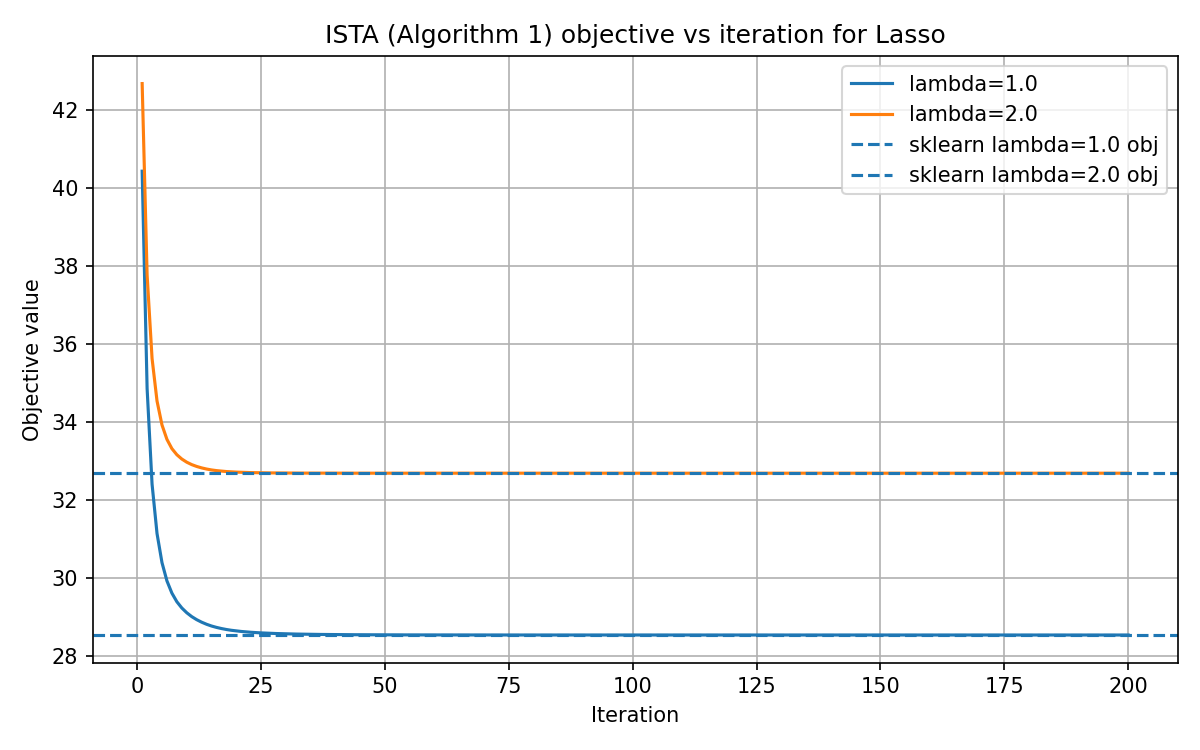
\includegraphics[width=0.7\textwidth]{lasso_ista_vs_sklearn.png}
\caption{Objective value vs iteration for ISTA with $\lambda=1$ and $\lambda=2$.}
\end{figure}

\subsection*{Part 2: Comparison with sklearn Lasso}

We compare the output of Algorithm 1 with the Lasso implementation in
\texttt{sklearn.linear\_model.Lasso}. To match the objective function,
we set $\alpha = \lambda / m$ where $m=100$.

The coefficient vectors from the two methods are very close.
For example,

\[
\|x_{\text{ISTA}} - x_{\text{sklearn}}\|_2 \approx 10^{-3}.
\]

The objective values are also nearly, if not exactly identical, which indicates that
Algorithm 1 converges to the same solution as the sklearn Lasso solver.

\end{document}